\scanpage{31}

\unsure{On a la} suite spectrale
\[
H^{\unsure{*|p+q}}(S,F)\Longleftarrow\varinjlim_{\unsure{\mathcal U|U}} H^p(\unsure{\mathcal U|U},H^q(F))=E_2^{pq}.
\]
et
\[
E_2^{pq}=0\quad\text{si}\quad p=0,\ q>0.
\]

\unsure{Car} \deleted{\unsure{prouve}}\inserted{implique} déjà $(ii)\Rightarrow(i)$, Or moyennant $(i)$, $(ii)$ et $(iii)$ sont équivalents, donc $(ii)\Rightarrow(iii)$. De même trivialement $(ii\text{ bis})\Rightarrow(ii)$ et $(iii\text{ bis})\Rightarrow(iii)$, \deleted{et \unsure{on a} $(ii)\Rightarrow(i)$}\inserted{donc $(ii\text{ bis})\Rightarrow(i)$}, et \deleted{\unsure{que nous}} moyennant $(i)$, $(ii\text{ bis})$ et $(iii\text{ bis})$ sont équivalents, \unsure{i.e. on a} $(ii\text{ bis})\Rightarrow(iii\text{ bis})$. Tout sera fait

\margin{\diagram{\begin{tikzcd}[column sep=small,row sep=large]
& (ii)\arrow[dl,Rightarrow]\arrow[dr,Rightarrow] && (ii\text{ bis})\arrow[ll,Rightarrow]\arrow[dr,Rightarrow]\arrow[d,phantom,"{\deleted{\Downarrow}}"] & \\
(i) && (iii)\arrow[ll,Rightarrow]\arrow[r,phantom,"{\deleted{\Longrightarrow}}"] & \deleted{\unsure{(iii\text{ bis})}} & (iii\text{ bis})\arrow[ll,Rightarrow]
\end{tikzcd}}}

si nous prouvons que $(iii)\Rightarrow(i)$. Récurrence sur $n$. Si $n\leq0$, c'est vide. Supposons $n>0$, et que c'est prouvé pour $n'<n$. Donc on sait déjà que
\[
H^i(F)=\overline H^i(F)\quad\text{pour}\quad\uuline{i<n}\quad\deleted{\text{et}}
\]
\deleted{\unsure{faut le prouver pour} $i=n$} sur des arguments $\in\mathcal M$, donc
\[
E_2^{pq}=0\quad\text{si}\quad\deleted{p+q\leq n+1\text{ et }q\ne0}\inserted{0<q\leq\uline{n-1}}.
\]
\deleted{Donc} Mais

\margin{\figure{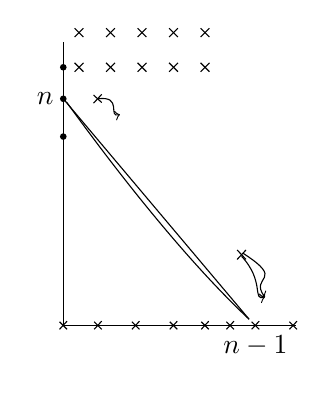
\begin{tikzpicture}[x=0.8cm,y=0.8cm]
\draw (0,0)--(3.7,0);\draw (0,0)--(0,4.5);
\foreach \x in {0,0.55,1.15,1.75,2.25,2.65,3.05,3.65}{\draw (\x-0.06,-0.06)--(\x+0.06,0.07);\draw (\x-0.06,0.06)--(\x+0.06,-0.06);}
\foreach \y in {3.0,3.6,4.1}{\fill (0,\y) circle (1.2pt);}
\foreach \x in {0.25,0.75,1.25,1.75,2.25}{\foreach \y in {4.1,4.65}{\draw (\x-0.07,\y-0.07)--(\x+0.07,\y+0.07);\draw (\x-0.07,\y+0.07)--(\x+0.07,\y-0.07);}}
\draw (0,3.6)--(2.95,0.1);\draw (0.05,3.55)..controls (1.1,2.1) and (2.1,0.9)..(2.95,0.1);
\node[left] at (0,3.6) {$\unsure{n}$};\node[below] at (3.05,0) {$n-1$};
\draw[->] (0.55,3.6)..controls (0.95,3.65) and (0.7,3.3)..(0.9,3.35);
\draw (0.48,3.53)--(0.61,3.67);\draw (0.48,3.66)--(0.61,3.54);
\draw[->] (2.85,1.15)..controls (3.55,0.7) and (2.95,0.8)..(3.2,0.45);
\draw[->] (2.83,1.1)..controls (3.2,0.7) and (3.0,0.4)..(3.2,0.45);
\draw (2.76,1.05)--(2.9,1.2);\draw (2.76,1.2)--(2.9,1.05);
\end{tikzpicture}}}

la suite spectrale donne
\[
\deleted{\unsure{H^n(S,F)}\simeq}
\]
\[
\varinjlim_{\unsure{\mathcal U|U}} H^n(\unsure{\mathcal U|U},F)\simeq H^n(S,F)
\]
\deleted{\unsure{d'où encore}} \deleted{$\unsure{H^n(F)}$} cqfd.

\uline{Schéma logique} \unsure{Résumons} les \unsure{4} implications ci-contre, plus le fait que
\[
(i)\Longrightarrow[(ii)\Rightarrow(iii)\text{ et }(ii\text{ bis})\Leftrightarrow(iii\text{ bis})]
\]
\margin{\diagram{\begin{tikzcd}[column sep=small,row sep=small]
(ii\text{ bis})\arrow[d,Rightarrow]\arrow[rr,phantom,"{\deleted{\unsure{\Longleftrightarrow}}}"] && (iii\text{ bis})\arrow[d,Rightarrow]\\
(ii)\arrow[dr,Rightarrow] && (iii)\arrow[dl,Rightarrow]\\
& (i) &
\end{tikzcd}}}
\mspage{30}

